\appendix
\section{Meetresultaten}
\label{appendix:meetresultaten}

In deze bijlage worden de meetresultaten weergegeven die zijn verzameld tijdens de experimenten.

\section{Tabel met resultaten}
Hieronder staat een overzichtstabel van de gemeten waarden.

\begin{table}[h!]
\centering
\begin{tabular}{|c|c|c|}
\hline
Tijd (s) & Spanning (V) & Stroom (A) \\
\hline
0.0 & 3.30 & 0.10 \\
1.0 & 3.28 & 0.11 \\
2.0 & 3.27 & 0.12 \\
\hline
\end{tabular}
\caption{Gemeten waarden tijdens test 1}
\end{table}

\section{Grafiek}
Hier zie je een voorbeeld van een grafiek (je moet je eigen figuur invoegen):

\begin{figure}[h!]
\centering
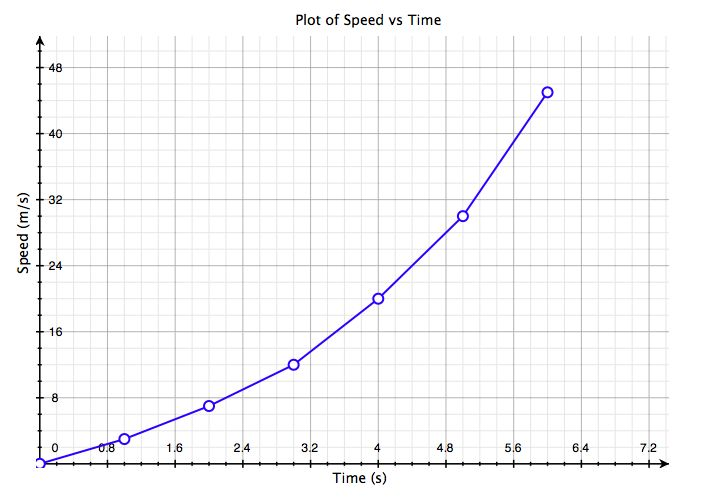
\includegraphics[width=0.7\textwidth]{./afbeeldingen/grafiek.jpeg}
\caption{Spanning over tijd}
\label{fig:spanning_tijd}
\end{figure}

\section{Broncode}
\label{appendix:broncode}

\section{Arduino-script}
\begin{lstlisting}[language=Python, numbers=left, breaklines=true, basicstyle=\ttfamily\scriptsize]
    def build_feedforward_model(input_layer_size, hidden_layer_size, output_layer_size):
        """Bouw een neuraal netwerkmodel volgens TensorFlow-conventies."""
        model = keras.Sequential(name="Feedfoward_Model")
        model.add(layers.Input(shape=(input_layer_size,), name="Input_Layer"))
        model.add(layers.Dense(hidden_layer_size, activation='sigmoid', name="Hidden_Layer"))
        model.add(layers.Dense(hidden_layer_size_2, activation='sigmoid', name="Hidden_Layer_2"))
        model.add(layers.Dense(output_layer_size, activation='softmax', name="Output_Layer"))
        return model 
    \end{lstlisting}
